\chapter{Microsoft Bot Framework}

The BotBuilder SDK is an open-source solution developed by Microsoft to write a chatbot once and make it possible to connect that same chatbot to multiple channels without rewriting the code. Examples are Skype, Slack, Facebook Messenger, etc.

\section{Business Model}

The Microsoft Bot Framework can be used in several ways. The base platform can be hosted on a server of choice. But to access the extra services, like spell checking, or recognizing user intents using Microsoft's LUIS (Language Understanding), an Azure subscription plan is required.

Azure is Microsoft's Cloud service that can be tailored to the customer's need. The customer can decide what modules or extra features he wants to add and calculate the price.

\begin{figure}[ht]
	\centering
	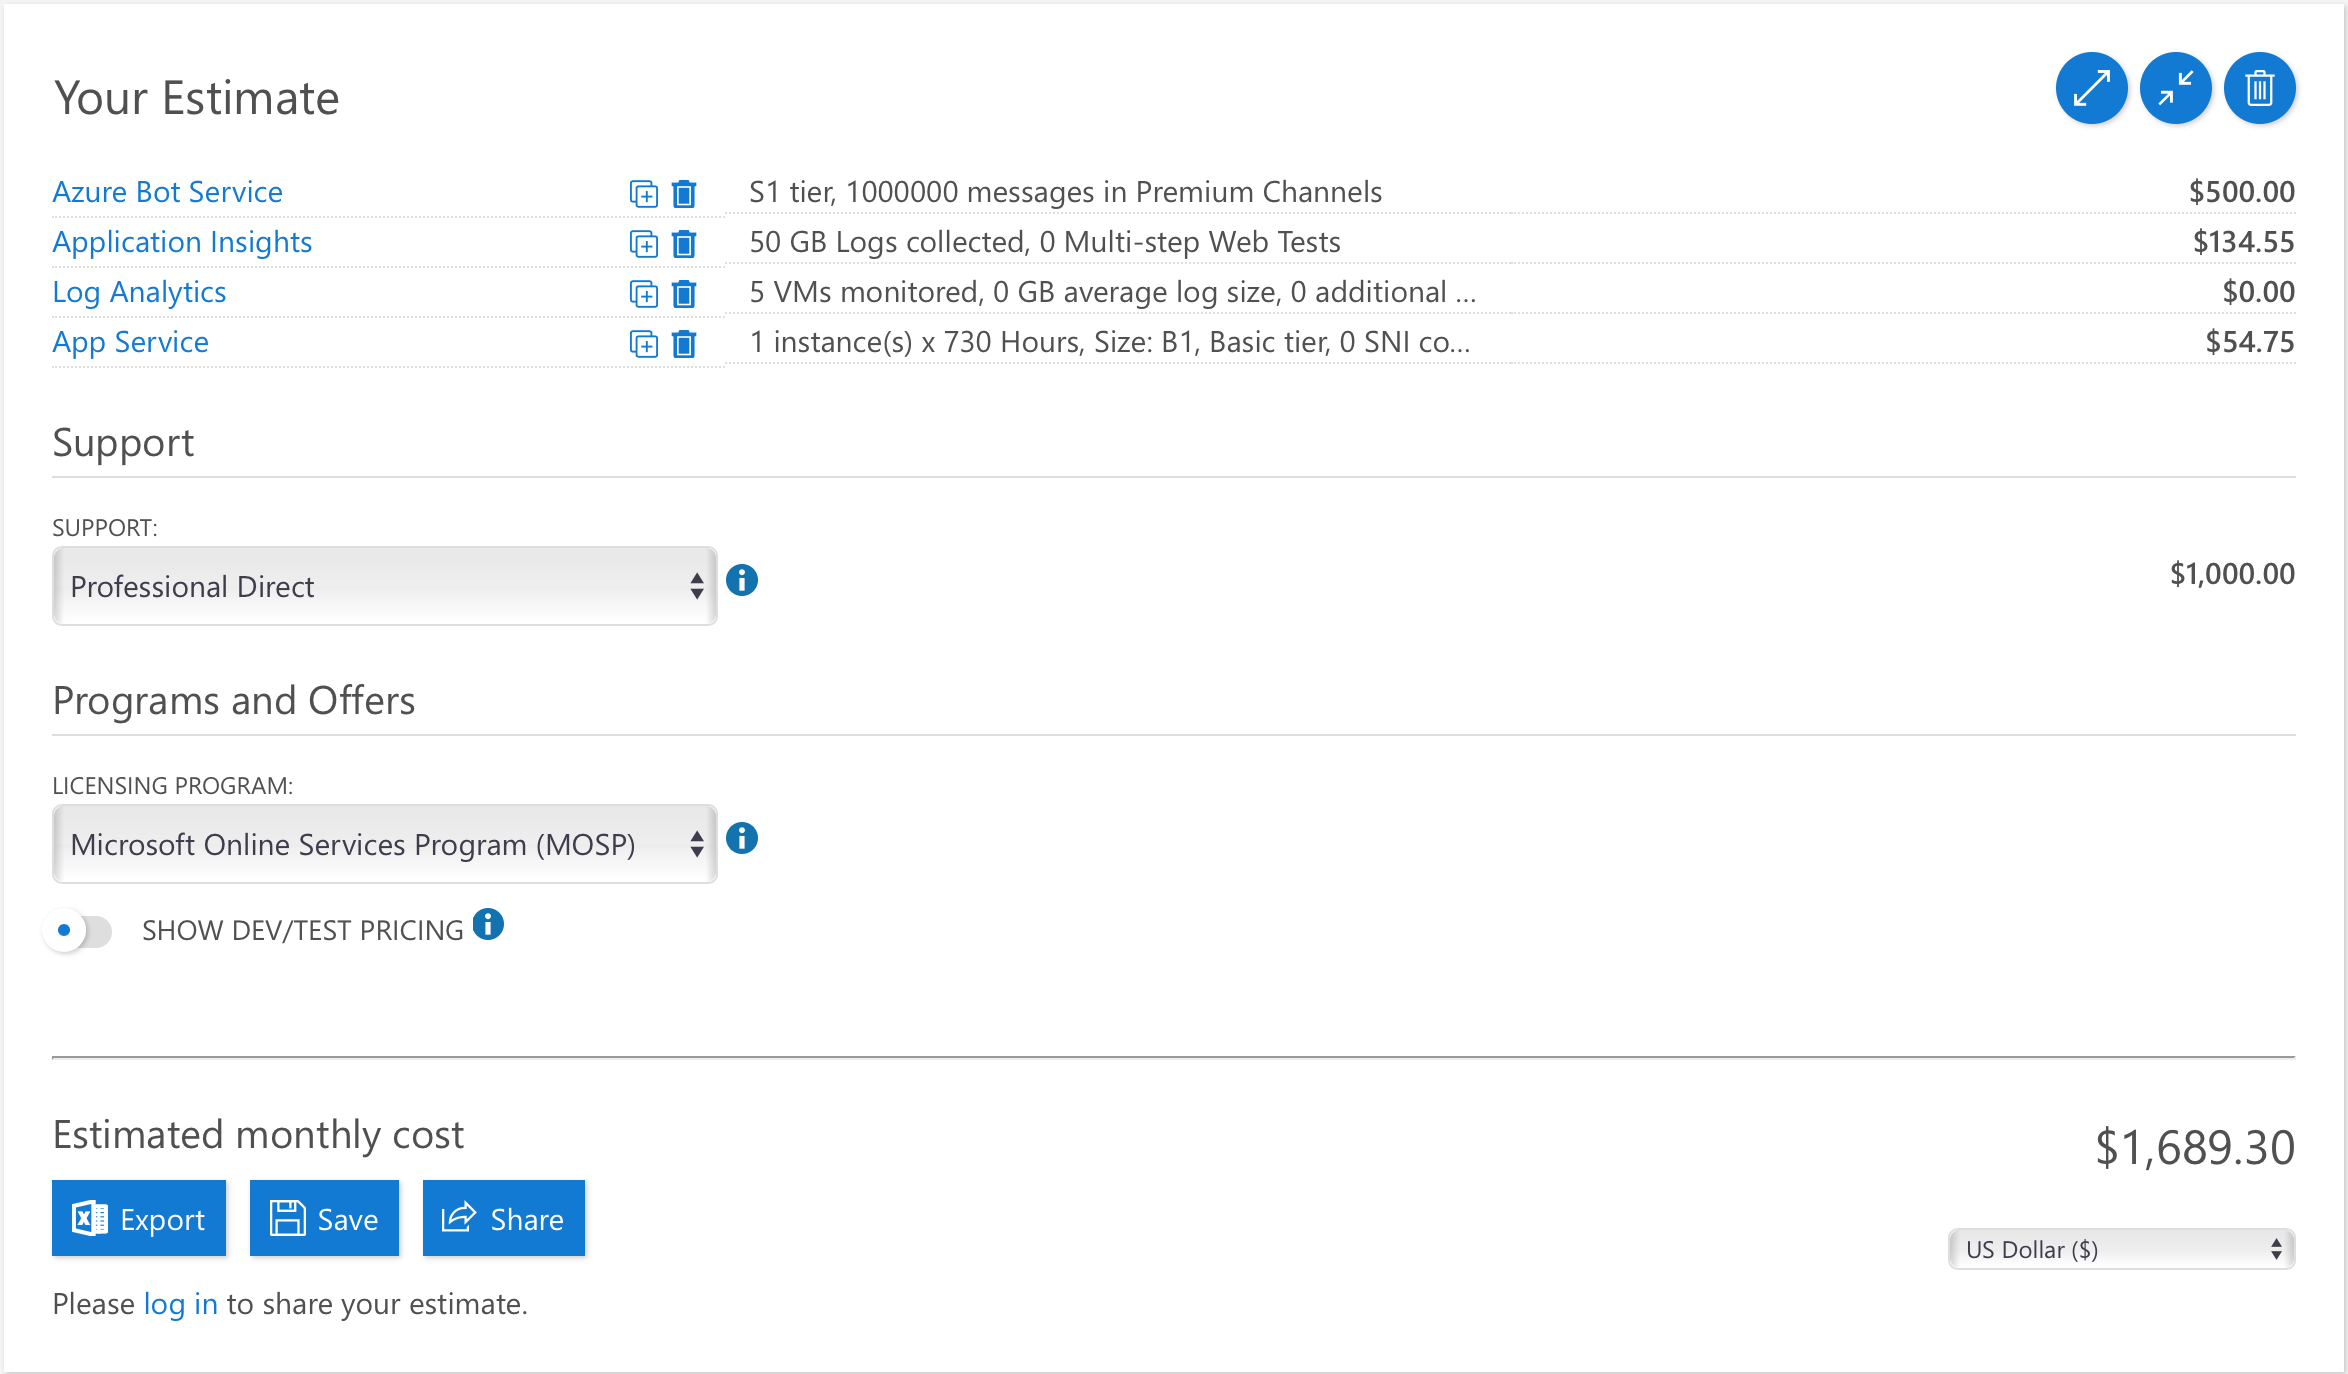
\includegraphics[width=\textwidth]{microsoft-azure-calculator-screen}\label{fig:microsoft-azure-calculator-screen}
	\caption{Microsoft's Azure Pricing Calculator~\cite{azure-pricing-calculator}}
\end{figure}

\section{Technical implementation}

Microsoft provides the bot framework for 2 languages: Node.JS\cite{node-js} and C\#. If C\# is used however, development can only be done inside of a Windows environment, or the limited online code editor.

One solution would be to use Node.JS in a code editor of choice. Preferably Visual Studio Code\cite{visual-studio-code}, Microsoft's cross-platform code editor. This way everything can be tailored and configured to the developer's needs.

\subsection{Developer environment}

Setting up a developer environment can be configured from scratch to be as complicated and complex as needed by the company or developer. Node.JS is an open-source, cross-platform JavaScript environment that can be run on a server. And in the end that's what a chatbot is, a server API that responds to requests (messages or events from the user).

It's important to note that JavaScript or also called \Gls{ECMAScript} is a language that is advancing very quickly and is rolling out yearly iterations. Currently the most recent iteration is called ES8. Node.JS is playing catch-up with these iterations and trying to support all of the additions.

The documentation involving the Bot Framework is written in \Gls{ES5}. But it's still possible to write everything in the most recent version of ECMAScript if you compile your code down. This process will turn your unsupported code into code that is supported by Node.JS, depending on the configuration.

Finding documentation on setting up an environment like this is not as easy as one would think. Microsoft does not provide any instructions or boilerplates on how to set up an efficient environment. This gives the developer more freedom but increases the learning curve for a someone who wants to start coding a bot using newer ECMAScript features or the option to hot-reload his code.

\subsubsection{Project structure}

Structuring the project is straight forward. Just like most production JavaScript projects there is a source folder containing all of the actual source code. Developers can decide to divide the test files into a separate folder but generally it's recommended to keep the test files close to the source file they refer to.

The node\_modules folder is a dependency folder, it contains any dependencies the project uses. There are two types of dependencies: First there are developer-dependencies, these are dependencies needed to build the project and participate in development. An example is ESLint\cite{eslint}, a configurable linter to make sure the source code follows specific language rules. There are also regular dependencies, these are external libraries the project might use to do calculations, or wrappers for certain technologies. The Microsoft Bot Framework functions using their botbuilder \Gls{SDK} as a dependency.

Next up are the configuration files, these are the workhorses of the developer's environment. They are used by Webpack\cite{webpack}. Webpack is a very powerful, well documented build tool and allows for easy customization. It is commonly used for front-end development but supports Node.JS development as well. The development config~\ref{appendix:botframeworkdevscript} starts a server that hot-reloads any changes made to the source files. This way it's easy for the developer to seamlessly check his changes instead of manually recompiling and restarting the server. The production config~\ref{appendix:botframeworkprodscript} compiles the code down to its most efficient format, which makes it unreadable to a developer, but very efficient for the production server to execute.

Further more there is support for environment variables using the dotenv\cite{dotenv} dependency. Variables can be securely stored in the env file, this file is not versioned to git and will contain any API keys used in the project.

\begin{figure}[ht]
	\centering
	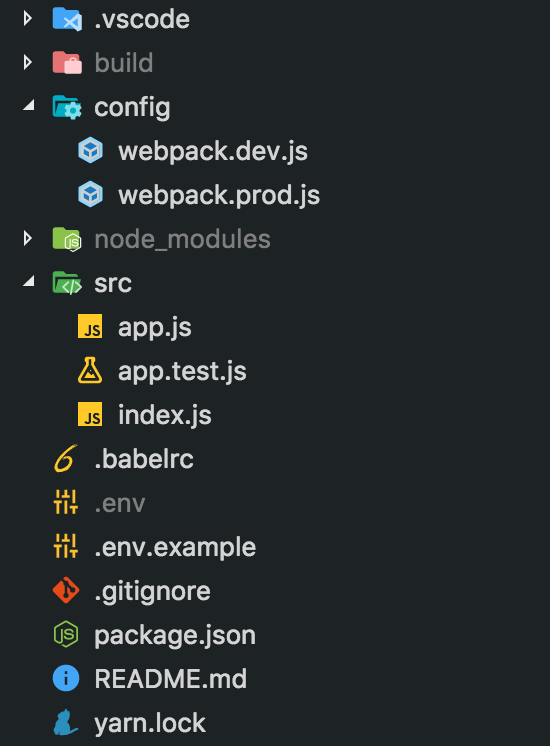
\includegraphics[width=0.33\textwidth]{projectstructure}\label{fig:projectstructure}
	\caption{Project structure}
\end{figure}

\subsection{Testing}

The bot can be tested locally or remotely on any platform using Microsoft's own Bot Emulator~\ref{fig:microsoft-bot-emulator}, which is also open-source. This provides the developer with a live testing interface and detailed information about the bot it's connected to.

It's possible to connect to a locally running bot, or a remotely hosted bot. Speech Recognition is supported for speech enabled bots. Sending system activities is another useful feature allowing the developer to emulate certain user actions like for example a user joining the conversation. Lastly, payment processing is supported to emulate a transaction.

A new iteration of the emulator makes it possible to write transcripts of a conversation in a simple format and load them into the emulator.

\begin{figure}[!hb]
	\centering
	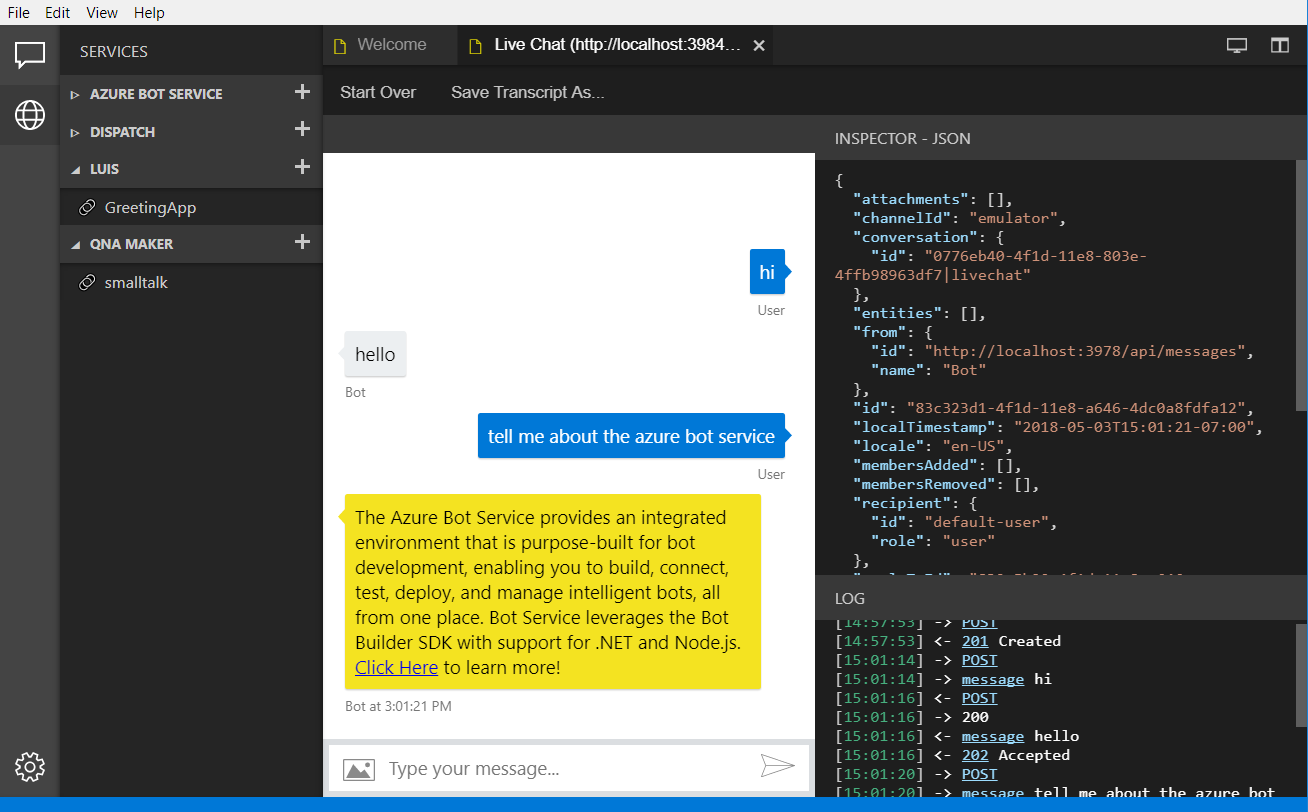
\includegraphics[width=\textwidth]{microsoft-bot-emulator}\label{fig:microsoft-bot-emulator}
	\caption{Microsoft's Bot Emulator~\cite{microsoft-bot-emulator}}
\end{figure}

\section{Building a bot}

\subsection{Initialization}

Initializing a bot is straightforward, the official documentation recommends restify\cite{restify} as the server. During initialization it's possible to define a default message the bot will always use as a reply if no other reply options match.

\begin{lstlisting}[language=JavaScript,caption=Initialization of a chatbot,label=listing:botframework-init]
import restify from 'restify';
import * as builder from 'botbuilder';

// Setup Restify Server
const server = restify.createServer();
server.listen(process.env.port || process.env.PORT || 3978, () => {
	console.log('%s listening to %s', server.name, server.url); 
});

// Create chat connector for communicating with the Bot Framework Service
const connector = new builder.ChatConnector({
		appId: process.env.MicrosoftAppId,
		appPassword: process.env.MicrosoftAppPassword
});

// Listen for messages from users 
server.post('/api/messages', connector.listen());

const bot = new builder.UniversalBot(connector, (session) => {
	session.send(
		"Sorry, I didn't get that. Type 'help' if you need assistance or try a different sentence.",
		session.message.text,
	);
}).set('storage', inMemoryStorage);
\end{lstlisting}

To make the bot start the conversation certain events can be used. In this case a `conversationUpdate' event will be used to trigger the root dialog.

\begin{lstlisting}[language=JavaScript,caption=The root event of a bot,label=listing:botframework-init-message]
bot.on('conversationUpdate', (message) => {
	if (message.membersAdded) {
		message.membersAdded.forEach((identity) => {
			if (identity.id === message.address.bot.id) {
				bot.beginDialog(message.address, '/welcome');
			}
		});
	}
});
\end{lstlisting}

\newpage

\subsection{Event types}
\begin{itemize}
	\item message
	\item conversationUpdate
	\item contactRelationUpdate
	\item typing
	\item ping
	\item deleteUserData
	\item endOfConversation
	\item event
	\item invoke
	\item messageReaction
\end{itemize}

During a regular conversation there are several different events that will be triggered. A message event simply represents any communication between bot and user. The conversationUpdate event is triggered when any members are added/removed from the conversation, including the bot. Or when conversation metadata has changed. The contactRelationUpdate event indicates that the bot was added to or removed from a user's contact list.
These are the most common events, the other events are pretty self-explanatory.

Most of these events can be manually triggered using the bot emulator or defined in code, enabling unit testing.

\begin{lstlisting}[language=JavaScript,caption=Sending a mock event to the bot,label=listing:botframework-mock-event]
const event = {
	address: { bot: { id: '0' }, user: { id: 0 } },
	agent: 'botbuilder',
	source: 'facebook',
	sourceEvent: '',
	type: 'conversationUpdate',
	membersAdded: [{ id: '0', isGroup: false, name: 'test' }],
	user: { id: '0', isGroup: false, name: 'test' },
};

connector.processEvent(event);
\end{lstlisting}

\section{Constructing a conversational flow}

One of the key concepts in the Bot Builder SKD are dialogs. Dialogs help the developer manage the conversational logic and is a fundamental part of developing a chatbot in the bot framework.

A dialog can be compared to a function. It can perform a specific task and be called at any point in time. Dialogs can also contain other dialogs to advance and branch off a conversation.

\subsection{Waterfall}

A waterfall is a type of dialog that guides the user through a set of steps or tasks. After each step, the bot will wait for the user to respond and pass the reply to the next step. A great example of this is ordering food. First the user will be asked for drinks, followed by the amount, again followed by the question for what starter the user wants, and so on. There is a clear structure the bot goes through, hence the name waterfall.

A waterfall is defined by creating an array of consecutive functions or waterfall steps inside of a dialog.

\subsubsection{Prompts}

To help the bot wait for a reply Microsoft provides developers with so called `Prompts'. These already contain some extra functionality to validate the user's reply. A prompt should be used whenever the bot expects a reply from the user.

\subsubsection{Types}

\begin{itemize}
	\item text
	\item confirm
	\item number
	\item time
	\item choice
	\item attachment
\end{itemize}

When used inside of a waterfall, the reply of the user will be passed to the next step using the `results' object. Another argument called `next' can be used as a method to skip to the next step of the waterfall.

\begin{lstlisting}[language=JavaScript,caption=2-step waterfall using a prompt,label=listing:waterfall-and-prompt]
bot.dialog('orderButtonClick', [
	(session) => {
		builder.Prompts.choice(session, 'Thirsty? Want to order any drinks?', 'Yes|No drinks', {
			listStyle: builder.ListStyle.button,
		});
	},
	(session, results, next) => {
		if (results.response.entity === 'Yes') {
			session.beginDialog('orderDrink');
		} else {
			next();
		}
	},
]);
\end{lstlisting}

\subsection{User actions}

There are multiple ways to handle user input other than the usage of prompts. One way of doing so is by using actions. Actions are bound to specific dialogs.

\subsubsection{Triggeraction}

The most common action is a `triggerAction'. This can be connected to a dialog to invoke it whenever the user inputs a matched term. Whenever this is triggered, the dialog stack is cleared and the invoked dialog will be the new first dialog on the stack.

This behavior isn't always desired when the conversation needs to be temporarily redirected and resumed later on. That's where the `onSelectAction' option comes in. This allows the developer to program different behavior to the action.

\begin{lstlisting}[language=JavaScript,caption=triggerAction being bound to a dialog and its behavior overwritten by onSelectAction,label=listing:triggerAction]
bot.dialog('help', function (session, args, next) {
	//Send a help message
	session.endDialog("Global help menu.");
})
// Once triggered, will start a new dialog as specified by
// the 'onSelectAction' option.
.triggerAction({
	matches: /^help$/i,
	onSelectAction: (session, args, next) => {
			// Add the help dialog to the top of the dialog stack 
			// (override the default behavior of replacing the stack)
			session.beginDialog(args.action, args);
	}
});
\end{lstlisting}

\subsubsection{BeginDialogAction}

A specific dialog can also be attached to a dialog using the `beginDialogAction' action. This can be useful to send the user to a contextual action. An example of this is when the user asks for specific help in a dialog context. When triggered, it will run the specified dialog and when that dialog finishes, resume at the step of the dialog it was bound to.

This is similar to calling the `session.beginDialog('dialogid')' method from inside any dialog.

\subsubsection{ReloadAction}

The reloadAction is somewhat self-explanatory. Binding this to a dialog means it will restart the dialog whenever the action is invoked.

\subsubsection{CancelAction}

This action cancels the dialog it is bound to when triggered. The parent dialog will also receive an indication the child dialog was canceled.

\subsubsection{EndConversationAction}

Similar to the cancelAction action, the endConversation action will end the entire conversation when triggered. This clears the entire dialog stack and persisted state data.

\subsubsection{CustomAction}

Unlike all the other actions, a customAction does not have any default action defined. It's up to the developer to define what it should do. The main benefit of using these is providing quick answers to a user without manipulating the dialog stack at all.

Further more a customAction does not bind to a dialog, instead it binds to the bot itself.

\subsubsection{Important to note}

Important to note is the fact that some of these actions are quite interruptive to the conversation's flow. To make sure the user really wants to clear the entire dialog stack and start over, a confirmation prompt can also be added to these actions.

\subsection{Messages}

There are many different kinds of messages the bot can send to the user. This ranges from the default text message to a fully constructed card with images or a video. However not all channels support fully constructed cards or other rich attachments.

\subsubsection{Channel Inspector}

The channel inspector~\cite{channel-inspector} is a tool developed by Microsoft to see what all of the message types look like on different platforms. A Skype card will different to a Messenger card for example. It also provides users with notes and limitations on a specific message type for a platform.

\begin{figure}[ht]
	\centering
	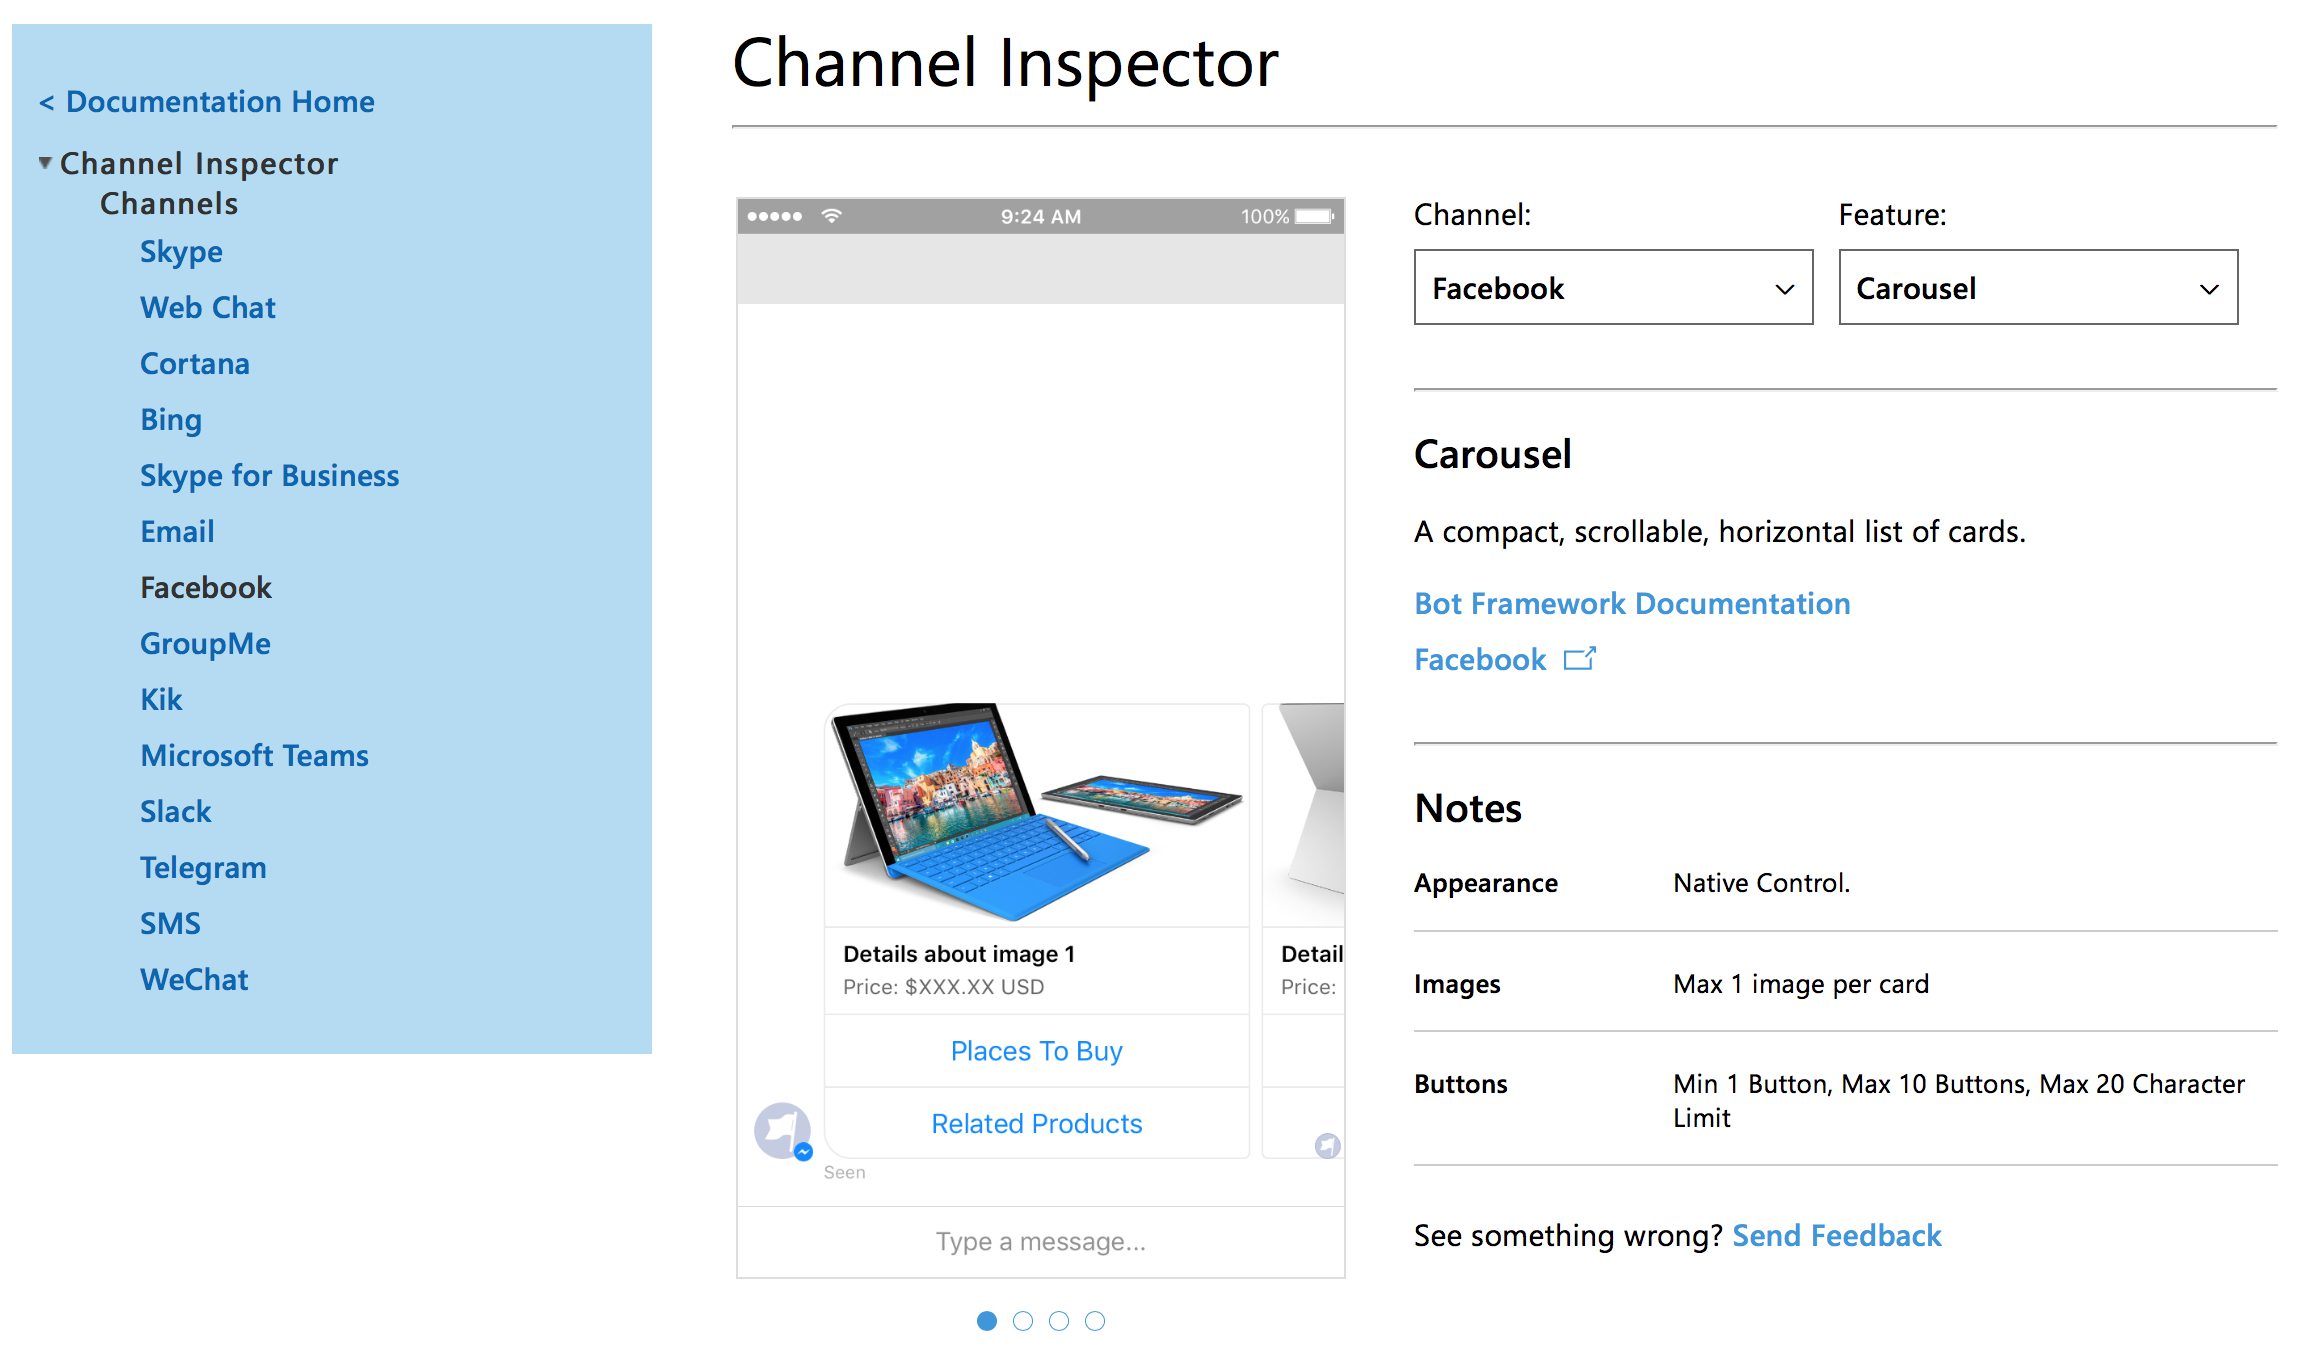
\includegraphics[width=\textwidth]{channel-inspector}\label{fig:channel-inspector}
	\caption{Channel Inspector}
\end{figure}

\subsubsection{Default message handler}

\begin{lstlisting}[language=JavaScript,caption=Sending a simple text message or reading the message from the user is very easy,label=listing:send-text-message]
session.send("Good morning.");

const userMessage = session.message.text;
\end{lstlisting}

To construct more complicated messages, a `Message' object will have to be created. After initialization, different methods can be called on the object to set properties, like attachments, input hints or even the format of the message.

\subsubsection{Attachments}

There are two main types of attachments that can be added to a message. There are media and files, this involves files like images audio or videos. A second type is a card. As seen in the example of the figure of the Channel Inspector~\ref{fig:channel-inspector}.

\begin{lstlisting}[language=JavaScript,caption=Receiving an attachment from the user and sending an image,label=listing:receive-attachment]
// Getting an attachment
const msg = session.message;
const attachment = msg.attachments[0];


// Sending a simple attachment
const attachment = {
	contentType: 'image/jpg',
	contentUrl: 'https://78.media.tumblr.com/tumblr_m1wmyyTckD1qejbiro1_500.jpg',
	name: 'This is definitely not a cat image',
});

session.send({
	text: 'Here is a cat image!',
	attachments,
});
\end{lstlisting}

\subsubsection{Cards}

Many different types of cards are available. Multiple cards can be added to a single message and displayed using a carousel, as seen in listing~\ref{listing:send-hero-card}.

\renewcommand{\arraystretch}{2}
\begin{table}[h]
	\centering
	\begin{tabular}{p{0.2\textwidth} |p{0.8\textwidth}}
		Hero Card      & The most common one, usually contains one big image, text and one or more buttons.             \\
		Thumbnail Card & Contains a single thumbnail, text and one or more buttons.                                     \\
		Animation Card & A card for gifs or short videos.                                                               \\
		Audio Card     & A card for an audio file.                                                                      \\
		Video Card     & A card for a video file.                                                                       \\
		Receipt Card   & A card that mimics a real receipt, allowing to input an item and cost, taxes, total cost, etc. \\
		Signin Card    & To request a user to sign in from a 3rd party                                                  \\
		Adaptive Card  & A fully customizable card that can contain images, text, input fields, buttons, etc.           \\
	\end{tabular}
	\caption{The different types of cards}
	\label{tab:card-types}
\end{table}

\begin{lstlisting}[language=JavaScript,caption={Example of how to construct some HeroCards and display them in a carousel},label={listing:send-hero-card}]
const cards = [
	new builder.HeroCard(session)
		.title(Item 1)
		.subtitle($5)
		.buttons([builder.CardAction.imBack(session, 'Item 1', 'Add to order')])
		.images([builder.CardImage.create(session, 'https://item-1.jpg')])),
	new builder.HeroCard(session)
		.title(Item 2)
		.subtitle($7)
		.buttons([builder.CardAction.imBack(session, 'Item 2', 'Add to order')])
		.images([builder.CardImage.create(session, 'https://item-2.jpg')])),
]

const msg = new builder.Message(session)
	.attachmentLayout(builder.AttachmentLayout.carousel)
	.attachments(cards);
\end{lstlisting}

The chatbot created for this case study makes use of the HeroCard to represent products. Each product has a title, price, image and button `Add to order'.

\newpage

\subsection{Storage}

Managing state data can be approached in several ways. State data could represent a user and its preferences over time, or it could be data that is only temporarily stored during the conversation, like the current order for a user.

Microsoft recommends the usage of the Bot Builder Framework's own in-memory data storage for testing and prototype bots. But for production bots they recommend the developers to implement their own storage solution, or use on of the Azure extensions to store data in \Gls{TableStorage}\cite{table-storage}, \Gls{CosmosDB}\cite{cosmosdb}, or SQL.

If one of the Azure integrations is implemented, the methods used to set and persist data are the same as the In-memory data storage.

\subsubsection{In-memory data storage, CosmosDB or Table Storage}

Important to note is the fact that this storage is cleared every time the bot is restarted, that is why it's only recommended for testing purposes.

\begin{lstlisting}[language=JavaScript,caption={Example on how to set up the in-memory data storage},label={listing:in-memory-storage}]
const inMemoryStorage = new builder.MemoryBotStorage();

const bot = new builder.UniversalBot(connector, [..waterfall steps..]).set('storage', inMemoryStorage);
\end{lstlisting}

As seen in listing~\ref{listing:in-memory-storage}, the storage is set when creating the bot instance. The setup when using one of the Azure extensions is very similar, the developer simply imports a package and sets some API keys before adding the storage to the bot.

\begin{table}[h]
	\centering
	\begin{tabular}{p{0.30\textwidth} | p{0.15\textwidth} | p{0.55\textwidth}}
		Container               & Scope        & Description                                                                           \\
		\hline
		userData                & User         & Data bound to user, persists across different conversations.                          \\
		privateConversationData & Conversation & Data bound to user, does not persist across conversations.                            \\
		conversationData        & Conversation & Data bound to a conversation, but shared across all users inside of the conversation. \\
		dialogData              & Dialog       & Data bound to a single dialog, when the dialog ends the data is cleared.
	\end{tabular}
	\caption{Storage containers}
	\label{tab:storage-containers}
\end{table}

As seen in table~\ref{tab:storage-containers} there are several different containers which can be used to store data. The `userData' container can be used to store user preferences and persist them across conversations. The `conversationData' and `privateConversationData' containers could be used to store the user's current order, as that is only relevant to the current conversation. The `dialogData' container is useful for data relevant to the dialog.

Setting or getting this data is as easy as it gets. Once set up, the containers can be accessed anywhere using the `session' object as seen in listing~\ref{listing:storage-containers}.

\begin{lstlisting}[language=JavaScript,caption={Example on how to use the storage containers},label={listing:storage-containers}]
// set data
session.userData.preferences = ['spicy']; 

// get data
const preference1 = session.userData.preferences[0];

// delete data
session.userData = {};
\end{lstlisting}
